\makeatletter
\def\input@path{{../}}
\makeatother

\documentclass[/main.tex]{subfiles}

\begin{document}
\graphicspath{{./pics/}{ch6/pics/}}

\onlyinsubfile{\textpages}
\chapter{Conclusion}
\section{Summary of Results}
The results presented in this dissertation represent the best limits to date for each \Ge{76} \bbes\ decay mode.
Meaningful constraints are placed on the value of the \bbes\ to the \SP{0}{+}{1} nuclear matrix element.
This chapter will place the results of this analysis in the context of previous results and theoretical predictions.
It will also discuss the potential for future improvements on this result.

\subsection{Comparison to \Gerda\ Phase I result}
\begin{table}[t]
  \centering
  \caption[Comparison between results from the \MJD\ and \Gerda]{\label{tab:mjdgerdacomp}
    A comparison between the key parameters behind the results for \MJD\ and \Gerda\ for each \tnbb\ to excited states mode. Backgrounds and efficiencies are combined across modules and peaks. Limits and sensitivities are at 90\% Neyman confidence level.
  }
  
  \begin{tabular}{|c|c c c c|c c c c|}
  \hline
  & \multicolumn{4}{c|}{The \MJD} & \multicolumn{4}{c|}{\Gerda} \\
  \makecell{\tnbb\ E.S. \\Decay Mode} & \makecell{Exp.\\BGs} & \makecell{Eff.\\(\%)} & \makecell{Limit\\($10^{23}$ y)} & \makecell{Sensitivity\\($10^{23}$ y)} & \makecell{Exp.\\BGs} & \makecell{Eff.\\(\%)} & \makecell{Limit\\($10^{23}$ y)} & \makecell{Sensitivity\\($10^{23}$ y)} \\
  \hline
  \decaySP{2}{0}{1} & 2.02 & 1.71 & $>6.8$ & $>7.0$ & 7.9 & 0.919 & $>3.7$ & $>1.9$ \\
  \decaySP{2}{2}{1} & 0.72 & 1.06 & $>9.6$ & $>5.3$ & 2.4 & 0.389 & $>1.6$ & $>1.3$ \\
  \decaySP{2}{2}{2} & 3.40 & 1.64 & $>5.6$ & $>5.3$ & 8.7 & 0.686 & $>2.3$ & $>1.4$ \\
  \hline
\end{tabular}
\end{table}
\Gerda\ phase I published the previous best results for all \tnbb\ decay modes in 2015, using 22.3~kg-y of exposure\cite{gerdaESresult}.
This result, using 21.3~kg-y of exposure has achieved a significantly higher sensitivity and limit.
\Gerda\ employed similar analysis techniques to this result, but the \MJD\ enjoys several advantages in performing searches in multi-site detectors.
First, the \Gerda\ liquid argon veto acts as shielding for $\gamma$s that travel between HPGe detectors.
A 600~keV $\gamma$ has a mean free path through liquid argon of ${\sim}9$~cm, and the spacing between different \Gerda\ strings is several cm, resulting in significantly lower detection efficiency compared to the \MJD.
For the decay to the \SP{0}{+}{1} state, \Gerda\ had a detection efficiency of 0.989~\%, while the \MJD\ had an efficiency of 1.71\%, exposure-averaged between the two modules.

\begin{figure}[h]
  \centering
  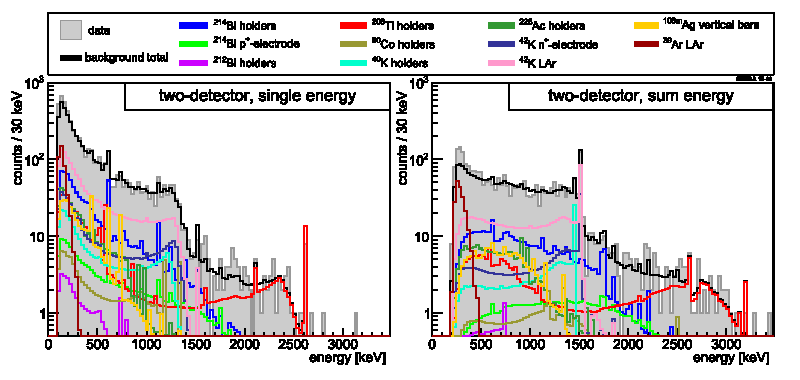
\includegraphics[width=0.9\textwidth]{gerdabackgrounds}
  \caption[\Gerda\ multi-site event backgrounds]{\label{gerdabgmodel}
    The measured \Gerda\ single-hit and sum-energy spectra for high multiplicity events compared with the measured data. The dominant background in this spectrum originates from \iso{42}{K} in the liquid argon shield. Taken from \cite{gerdaESresult}.
  }
\end{figure}
In addition, \Gerda\ has a significantly higher background rate in the ROI: for the decay to the \SP{0}{+}{1} state, \Gerda\ expects 7.9~background counts while the \MJD\ expects 2.02~counts.
One reason for this, is that the \MJD\ has significantly better resolution: the FWHM for a  583~keV coincident $\gamma$ is 1.3~keV for the \MJD, and 4.2~keV for \Gerda.
Electronic crosstalk in the \Gerda\ detector array increases the FWHM from 3.8~keV to 4.2~keV.
The LMFE boards (Section~\ref{sec:signalelectronics}) and their proximity to the \MJ\ detectors provide low noise and minimal crosstalk (Section~\ref{sec:crosstalk}), and the charge trapping correction (Section~\ref{sec:energy}) provides further improvements.
As a result, the \MJD\ uses separate ROIs for the 559~and 563~keV $\gamma$s that combine to a width of 3.3~keV, while \Gerda\ uses a single 8.5~keV wide ROI.
This explains most of the difference in background rates between the experiments; if \Gerda\ had the same ROI, the expected background rate would reduce to 3.1~counts.
Additionally, the dominant background for \Gerda\ in this search comes from \iso{42}{K} from the \iso{42}{Ar}-\iso{42}{K}-\iso{42}{Ca} chain inside of the liquid argon shield (see Figure~\ref{gerdabgmodel}).
Because this decay can emit $\gamma$s from the interior of the detector array, it will produce multi-site events with high enough energies to pass the coincident energy cuts at a relatively high rate.
This likely explains the remaining difference between the background rates.

Since publishing the phase~I result\cite{gerdaESresult}, \Gerda\ has implemented numerous improvements that may improve on the previous result\cite{gerda2018}.
\Gerda\ phase~II has since replaced many coaxial HPGe detectors with BEGe detectors, which are smaller, resulting in a more granular array that will be more sensitive to multi-detector events.
Additionally, the liquid argon shield has been instrumented, enabling it to act as an active shield, which may reduce backgrounds, and potentially could be used to detect $\gamma$s from the excited state decays.
\iso{42}{K} backgrounds are expected to be reduced with the addition of protective shrouds around detectors.
Finally, improvements to the signal electronics and corrections for detector crosstalk may be implemented to improve the energy resolution.

\subsection{Comparison to Theoretical Predictions}
\begin{table}[p]
  \caption[Current half-live limits and predictions for all \tnbb-decay modes of \Ge{76}]{\label{tab:Ge76HalfLives}
    Table of theoretical half-life predictions for each \tnbb\ decay mode
  }
  \small
  \begin{tabular}{|c|r|c c c|}
  \hline
  \tnbb\ Decay Mode & $T^{2\nu\beta\beta}_{1/2}$~(yr) & Experiment/Model & ref. & year \\
  \hline\hline
  \multirow{9}{*}{\makecell{\decaySP{2}{0}{1} \\ \Qbb$=916.8$~keV \\ $559.1 + 563.2$~keV~$\gamma$}}
  & $>6.8\e{23}$ & MJD & \ref{tab:allresults} & 2019 \\
  \cline{2-5}
  & $4.0\e{22}$       & QRPA & \cite{Civitarese1994} & 1994 \\
  & $4.5\e{22}$       & QRPA & \cite{Stoica1996} & 1996 \\
  & $7.5\e{21}$       & MCM-QRPA & \cite{Suhonen1996} & 1996 \\
  & $(1.0-3.1)\e{23}$ & RQRPA & \cite{Suhonen1997} & 1997 \\
  & $(1.2-5.8)\e{23}$ & RQRPA & \cite{gerdaESresult} & 2014 \\
  & $(6.0-6.1)\e{24}$ & IBM-2 & \cite{barea2013, barea2015} & 2014 \\
  & $(2.3-6.7)\e{24}$ & SM & \cite{gerdaESresult} & 2014 \\
  & $1.5\e{24}$       & ET & \cite{menendez2018} & 2018 \\
  \hline\hline
  \multirow{9}{*}{\makecell{\decaySP{2}{2}{1} \\ \Qbb$=1480.0$~keV \\ $559.1$~keV~$\gamma$}}
  & $>9.6\e{23}$ & MJD & \ref{tab:allresults} & 2019 \\
  \cline{2-5}
  & $1.2\e{30}$ & SM & \cite{Haxton1984} & 1984 \\
  & $5.8\e{23}$ &  HFB & \cite{dhiman1994} & 1994 \\
  & $5.0\e{26}$ & QRPA & \cite{Civitarese1994} & 1994 \\
  & $2.4\e{24}$ & QRPA & \cite{Stoica1996} & 1996 \\
  & $7.8\e{25}$ & MCM-QRPA & \cite{Suhonen1996} & 1996 \\
  & $1.0\e{26}$ & RQRPA & \cite{Suhonen1997} & 1997 \\
  & $(2.4-4.3)\e{26}$ & RQRPA & \cite{Simkovic1998} & 1998 \\
  & $5.75\e{28}$ & pnQRPA & \cite{Raduta2007} & 2007 \\
  & $2.0\e{27}$ & RQRPA & \cite{Unlu2014} & 2014 \\
  & $8.6\e{26}$ & ET & \cite{menendez2018} & 2018 \\
  \hline\hline
  \multirow{4}{*}{\makecell{\decaySP{2}{2}{2} \\ \Qbb$=822.0$~keV \\ $64\%: 657.0+559.1$~keV~$\gamma$ \\ $36\%: 1216.1$~keV~$\gamma$}}
  & $>5.6\e{23}$ & MJD & \ref{tab:allresults} & 2019 \\
  \cline{2-5}
  & $1.0\e{29}$ & QRPA & \cite{Civitarese1994} & 1994 \\
  & $1.3\e{29}$ & MCM-QRPA & \cite{Suhonen1996} & 1996 \\
  & $(0.7-2.2)\e{28}$ & RQRPA & \cite{Suhonen1997} & 1997 \\
  \hline
  
\end{tabular}

\end{table}
Table~\ref{tab:Ge76HalfLives} contains a list of theoretical predictions of the half-life of each \tnbb\ excited state decay mode for \Ge{76}.
The models presented include Hartree-Fock-Bogoliubov (HFB), Quasi-Random Phase Approximation (QRPA), Multiple Commutator Model QRPA (MCM-QRPA), Renormalized proton-neutron QRPA (RQRPA), Interactiing Boson Model (IBM), Shell Model (SM), and  Effective Field Theory (EFT) (recall Section~\ref{sec:NMEmethods}).
For some references included in Table~\ref{tab:Ge76HalfLives}, half-lives were not provided (the IBM\cite{barea2013, barea2015} and EFT\cite{menendez2018}); in these cases, the half-life provided was calculated using:
\begin{equation} \label{eq:hlcalc}
  T^{2\nu~E.S.}_{1/2} = T^{2\nu~G.S.}_{1/2}\cdot\frac{G_{2\nu}^{G.S.}|M_{2\nu}^{G.S.}|^2}{G_{2\nu}^{E.S.}|M_{2\nu}^{E.S.}|^2}
\end{equation}
where $T_{1/2}^{2\nu~g.s.}=1.926\pm0.094\cdot10^{21}$~y is the ground state decay half-life measured by \Gerda\ Phase~I.
$\mathrm{G}_{2\nu}$ are the phase space factors from Mirea, \textit{et al.}\cite{mirea2015}, and $|M_{2\nu}|$ are the matrix elements reported by the given source.
The EFT calculations\cite{menendez2018} also provided error estimates, which tend to be $40-80\%$ for excited state decays and are not shown here.

For each decay mode, the range of half life prediction spans many orders of magnitude.
This wide range is related to a variety of factors, including the method used to compute the matrix elements and model assumptions made about the intermediate nuclear states, the final nuclear states, $g_A$ quenching and the phase space integrals.
Because of the large number of factors that affect these calculations, it is difficult to draw conclusions about the different models based on a comparison to an experimental result.
Nevertheless, we shall perform such a comparison: the 90\% limit presented in this document rules out all predictions made with QRPA-based models for the \tnbb\ to \SP{0}{+}{1} state (the largest prediction by Suhonen\cite{gerdaESresult}, calculated assuming a $g_A$ factor of 1.27, is disfavored with a p-value of 0.08).
For the \tnbb\ to \SP{2}{+}{1} state the HFB prediction by Dhiman and Raina\cite{dhiman1994} is newly ruled out.
The \tnbb\ to \SP{2}{+}{2} state remains firmly out of reach of experiments.
For the \znbb\ decay modes, a meaningful comparison between experiment and nuclear theory calculations is not possible until the \znbb\ to the ground state is observed.
In addition, it is difficult to predict how an error in the prediction of any \tnbb\ to excited state half-life might correlate with an error in the \znbb\ half-life predictions, for reasons discussed in Section~\ref{sec:bbestheory}.
Improvements in some of the existing models presented in Table~\ref{tab:Ge76HalfLives} and future models can use excited state results as an additional test.
Ideally, they will agree with a measured result of the excited state decay half-lives, and predict similar values of the \znbb\ nuclear matrix elements, with measurements across multiple isotopes.
Table~\ref{tab:allisos} shows the current status of searches for \tnbb\ to \SP{0}{+}{1} states across multiple isotopes.
For a more complete discussion, see Barabash's review \cite{barabash2017}. 
\begin{table}
  \centering
  \caption[Table of \tnbb\ to \SP{0}{+}{1} states across multiple isotopes]{\label{tab:allisos}
    Table of results and predictions for the half-life of \tnbb\ to \SP{0}{+}{1} states across multiple isotopes. For the RQRPA results, half-lives were calculated within the references; for the IBM and EFT results, they were calculated using equation~\ref{eq:hlcalc}.
  }
  \begin{tabular}{|c|c|c c c|}
  \hline
   & Experiment & \multicolumn{3}{c|}{Theoretical $T^{2\nu~E.S.}_{1/2}$ (y)}\\
  Isotope & $T^{2\nu~E.S.}_{1/2}$ (y) & RQRPA\cite{Suhonen1997, suhonen2015} & IBM\cite{barea2015} & EFT\cite{menendez2018}\\
  \hline
  \iso{48}{Ca}  & $>1.5\cdot10^{20}$ \cite{Bakalyarov2002} & - & $2.0\cdot10^{23}$ & - \\
  \iso{76}{Ge}  & $>6.8\cdot10^{23}$ & $(1.0-3.1)\cdot10^{23}$ & $7.1\cdot10^{24}$ & $1.7\cdot10^{24}$ \\
  \iso{82}{Se}  & $>3.4\cdot10^{22}$ \cite{beeman2015} & $(1.5-3.3)\cdot10^{21}$ & $4.1\cdot10^{23}$ & $4.5\cdot10^{22}$ \\
  \iso{96}{Zr}  & $>3.1\cdot10^{20}$ \cite{finch2015} & $(2.4-3.8)\cdot10^{21}$ & $3.0\cdot10^{24}$ & - \\
  \iso{100}{Mo} & $6.7^{+0.5}_{-0.4}\cdot10^{20}$ \cite{barabash2017} & $(0.81-4.1)\cdot10^{22}$ & $5.7\cdot10^{21}$ & $5.2\cdot10^{20}$ \\
  \iso{116}{Cd} & $>2.0\cdot10^{21}$ \cite{piepke1994} & $(1.6-3.3)\cdot10^{24}$ & $8.4\cdot10^{23}$ & $1.8\cdot10^{23}$\\
  \iso{130}{Te} & $>2.5\cdot10^{23}$ \cite{adams2018} & $(7.2-16)\cdot10^{23}$ & $3.0\cdot10^{25}$ & $2.8\cdot10^{25}$\\
  \iso{136}{Xe} & $>8.3\cdot10^{23}$ \cite{asakura2015} & $(1.3-8.9)\cdot10^{23}$ & $3.0\cdot10^{25}$ & - \\
  \iso{150}{Nd} & $1.2^{+0.3}_{-0.2}\cdot10^{20}$ \cite{barabash2017} & - & $1.9\cdot10^{21}$ & - \\
  \hline
\end{tabular}
\end{table}

\section{The Future of \bbes\ in \Ge{76}}
The \MJD\ has been continuously acquiring data since the April~18, 2018 cutoff used in this analysis, and will continue to do so until it has a projected ${\sim}100$~kg-y of exposure.
In addition, much of the data-taking period remains to be unblinded, which increases the available exposure before the cutoff to ${\sim}40$~kg-y.
This increase in exposure should increase the sensitivity to the \bbes\ to the \SP{0}{+}{1} state half-life above $10^{24}$~y, potentially enabling a test of the EFT prediction of $1.7\cdot10^{24}$~y\cite{menendez2018}.

\subsection{Potential Improvements}
In addition to gathering additional exposure, other improvements to this search are possible.
In particular, the AvsE parameter, which is used to determine whether a waveform within a single detector is multi-site or single-site (see Section~\ref{sec:avse}), may be useful.
When a $\gamma$ is fully absorbed within a single detector, it will typically be detected as a multi-site event, while most Compton continuum events are single-site.
For example, the 583~keV $\gamma$ from the \Th{228} spectrum is ${\sim}75\%$ multi-site, while the Compton continuum is only ${\sim}41\%$ multi-site, as shown in Figure~\ref{fig:avse583}.
If the peak search were to only look at multi-site events, it would likely produce a small gain of up to ${\sim}20\%$ in sensitivity.
\begin{figure}[tb]
  \centering
  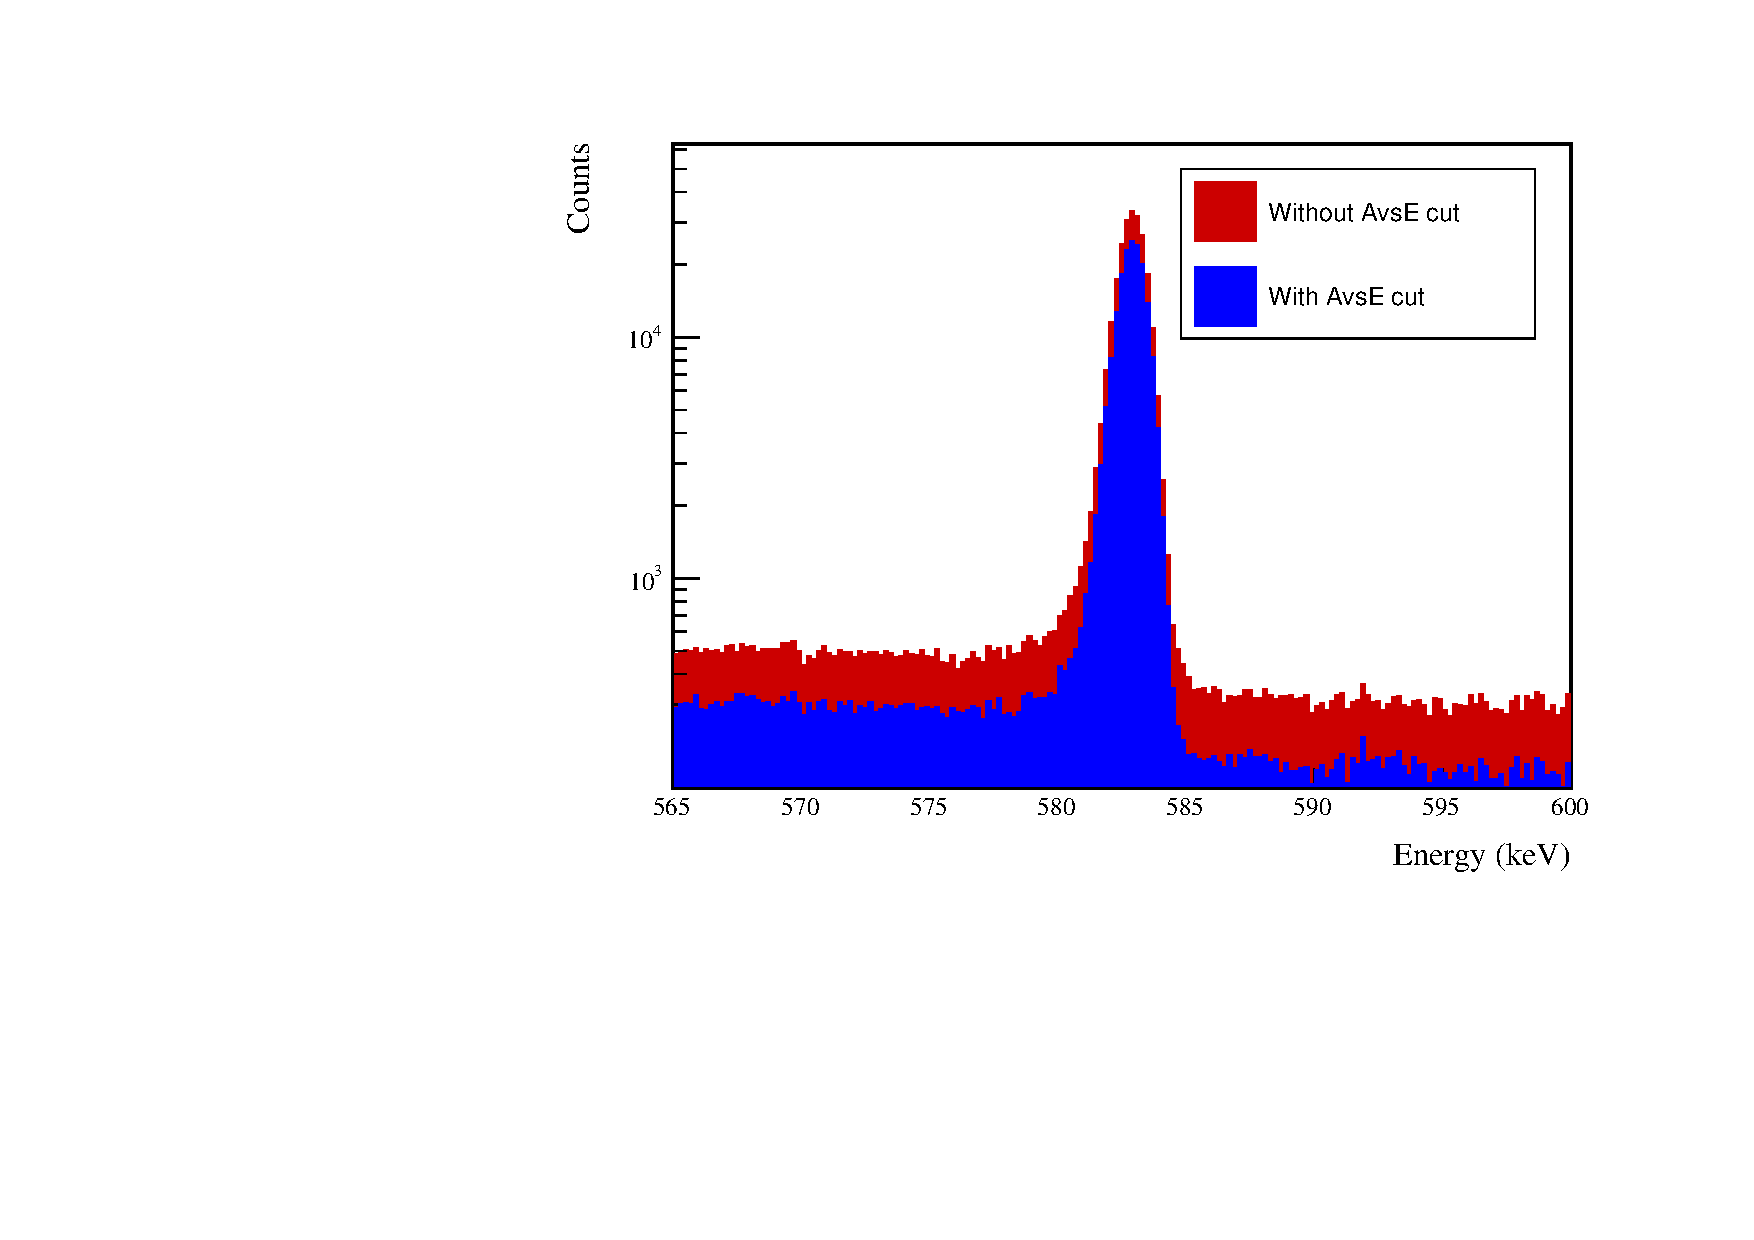
\includegraphics[width=0.6\textwidth]{avse583}
  \caption[583~keV peak with AvsE cut applied]{\label{fig:avse583}
    A 583~keV peak from a \Th{228} calibration run using AvsE to select multi-site events (blue). The effect is to keep 75\% of events in the peak while keeping only 41\% of events in the continuum.
  }
\end{figure}

The coincident energy cut could also benefit from using AvsE.
For decay modes with only a single $\gamma$ (such as the \SP{2}{+}{1} modes), the coincident detector in a true signal will have only a single site, from the \bb -decay.
On the other hand, for events with multiple $\gamma$s, coincident events with energy above the \Qval\ of the decay will result from events involving the internal absorption of one of the $\gamma$s; as a result, these events will be inherently multi-site.
Using AvsE in this cut will be especially important for differentiating between \SP{2}{+}{1} and \SP{0}{+}{1} events since they both involve a 559~keV peak.
This means that some method of differentiating between events involving one and two $\gamma$s will be critical to differentiating events in this peak, and AvsE may provide the best way of doing so.
A simulation of the effect of AvsE on the coincident energy spectrum is shown in Figure~\ref{fig:coincavse}.
\begin{figure}[tb]
  \centering
  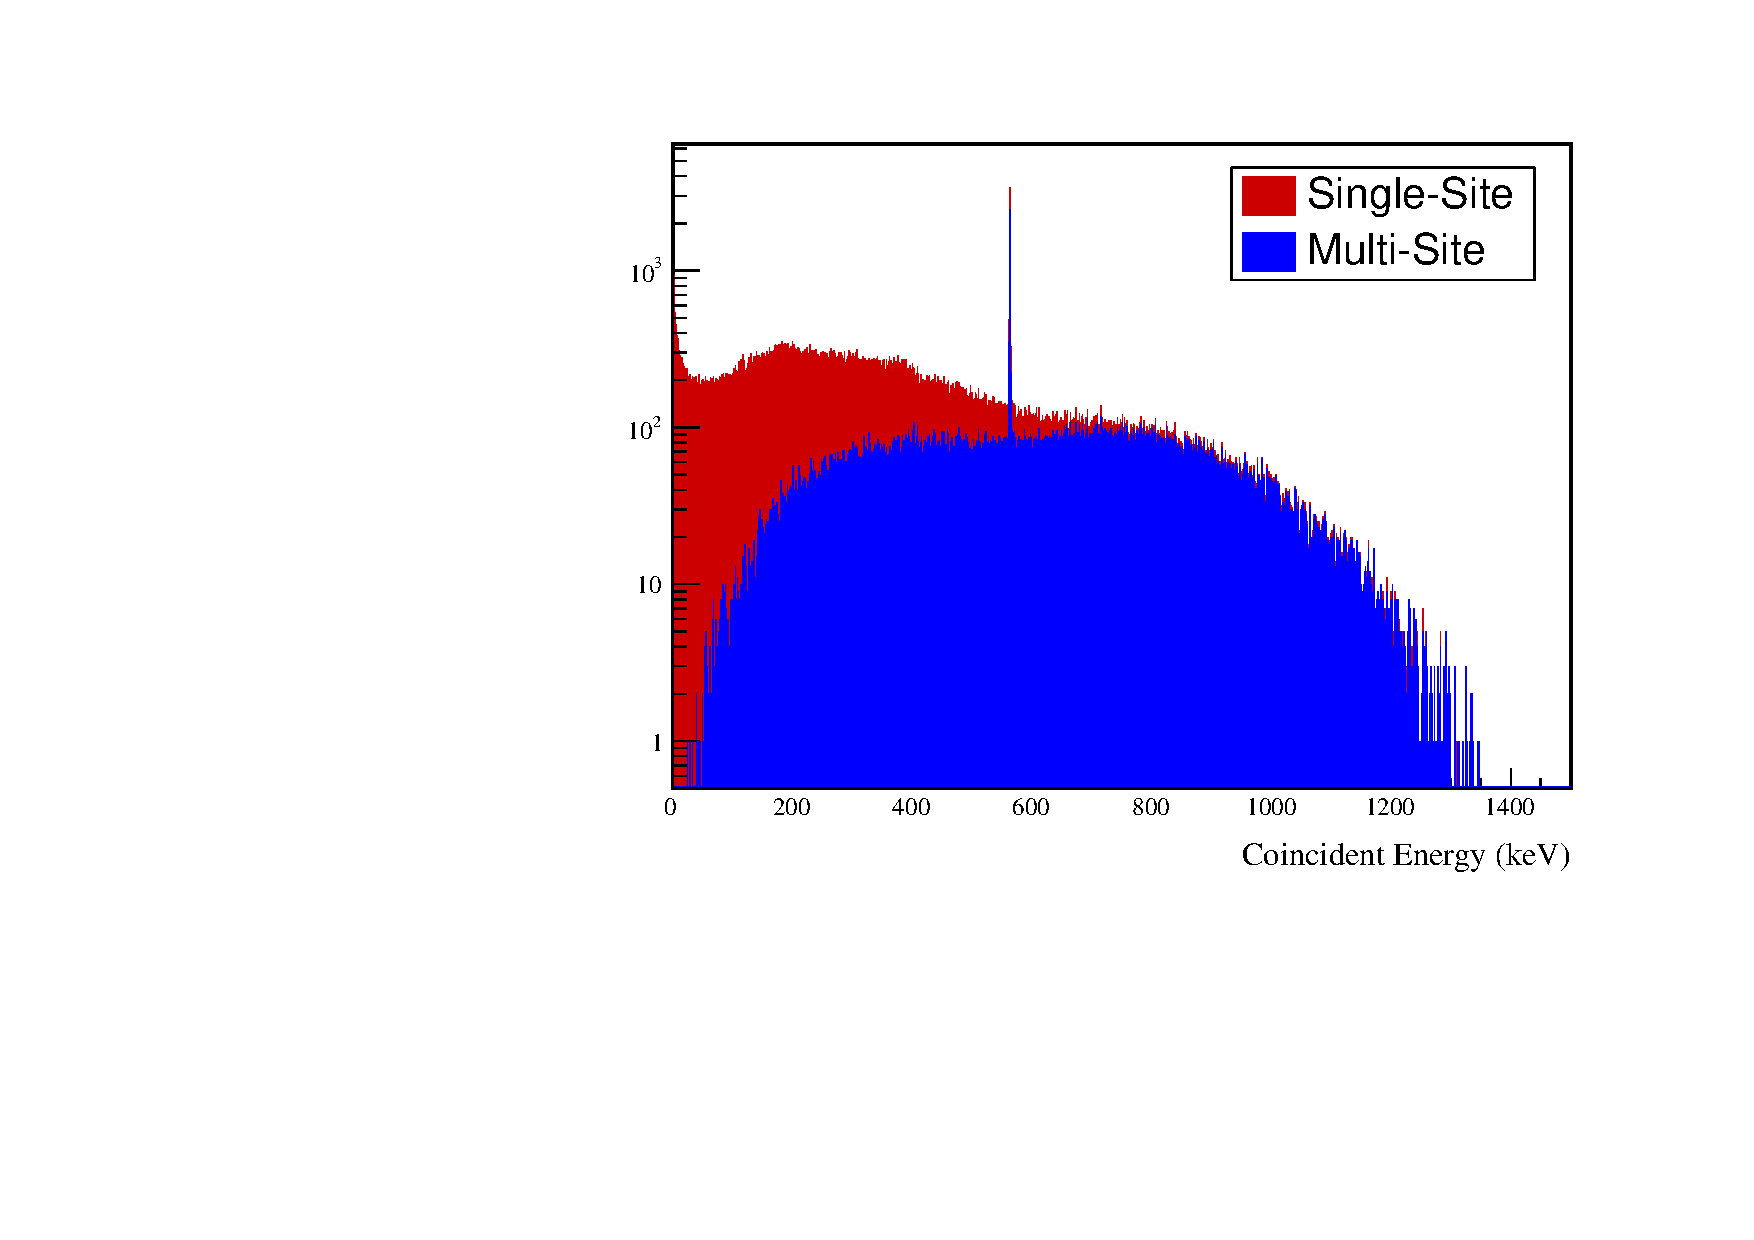
\includegraphics[width=0.6\textwidth]{coincidentcutwithavse}
  \caption[Coincident energy spectrum with multi-site event cut]{\label{fig:coincavse}
    Simulated energy spectrum for hits in coincidence with a 559~or 563~keV $\gamma$ from a \tnbb\ to \SP{0}{+}{1} event. The dt-heuristic was applied to simulate the effect of an AvsE cut.
  }
\end{figure}
The reason AvsE is not currently used for this search is that it cannot be simulated reliably.
The current method of simulating this parameter, called the dt-heuristic, is calibrated over an energy range close to 2039~keV, and has a relatively high error at the energies of interest for this analysis.
Since this analysis relies heavily on uncertain simulations that would introduce significant systematic error, and since the improvements brought by using AvsE are expected to be small, this cut was not used for this analysis.
However, further improvements to the dt-heuristic and development of pulse-shape simulations that can improve AvsE simulation may allow the implementation of this cut in the future.

  \subsection{Multi-Site Event Decomposition}
\begin{figure}[h]
  \centering
  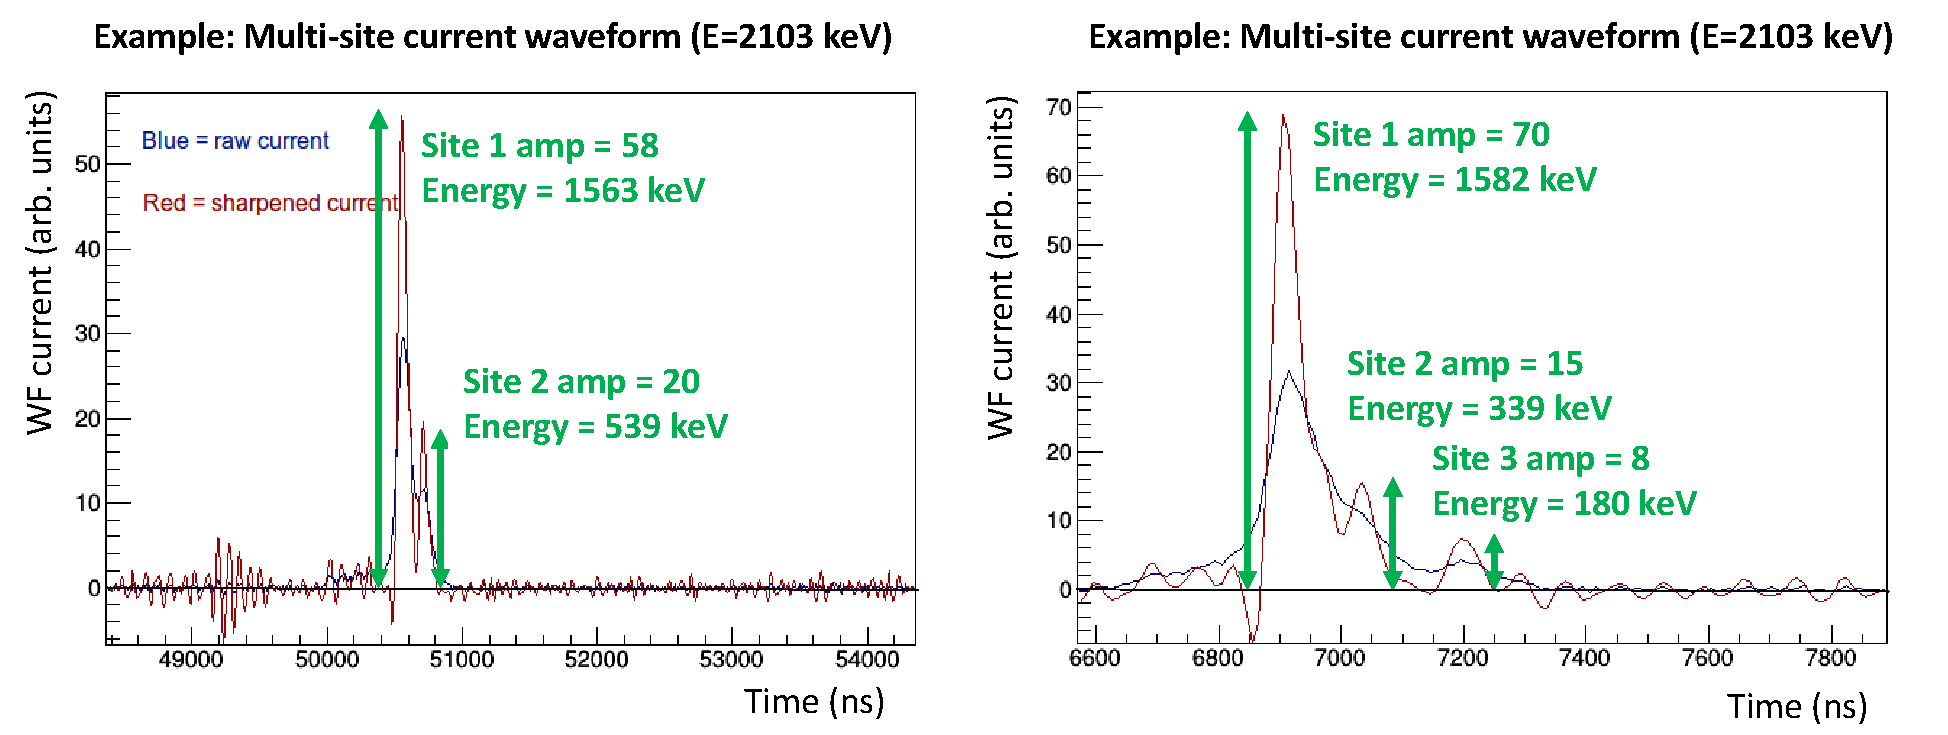
\includegraphics[width=\textwidth]{wienercurrent}
  \caption[Proof of principle for multi-site event decomposition]{\label{fig:wienercurrent}
    A Wiener deconvolution of two current waveforms with a Lorentzian deconvolution kernel. The current peaks can be identified and their amplitudes calibrated to measure energy. The waveforms were selected from the SEP and are expected to have a site with 1592~keV of energy.
  }
\end{figure}
In addition to distinguishing between single- and multi-site events, PPC HPGe detectors offer the possibility to decompose a multi-site waveform and measure the energies of the component sites.
Multi-site waveforms consist of multiple rises, as discussed in Section~\ref{sec:avse}, and the current amplitude of each individual rise is proportional to the energy contained in the local charge cloud producing it.
This proportionality is the reason the AvsE parameter works: for a single-site, the maximum current amplitude should be some fixed fraction of the total energy, while for multi-site waveforms, the current amplitude will be significantly less.
Due to electronic noise, however, picking out individual components of waveforms and measuring the energy with each one is difficult.
One method that has been demonstrated for doing this is to apply a Wiener deconvolution filter, which uses deconvolution with a known kernel function in order to sharpen the current peaks, combined with an optimal Wiener filter to prevent noise from blowing up.
A proof of principle for this technique is shown in Figure~\ref{fig:wienercurrent}.

\begin{figure}[h]
  \centering
  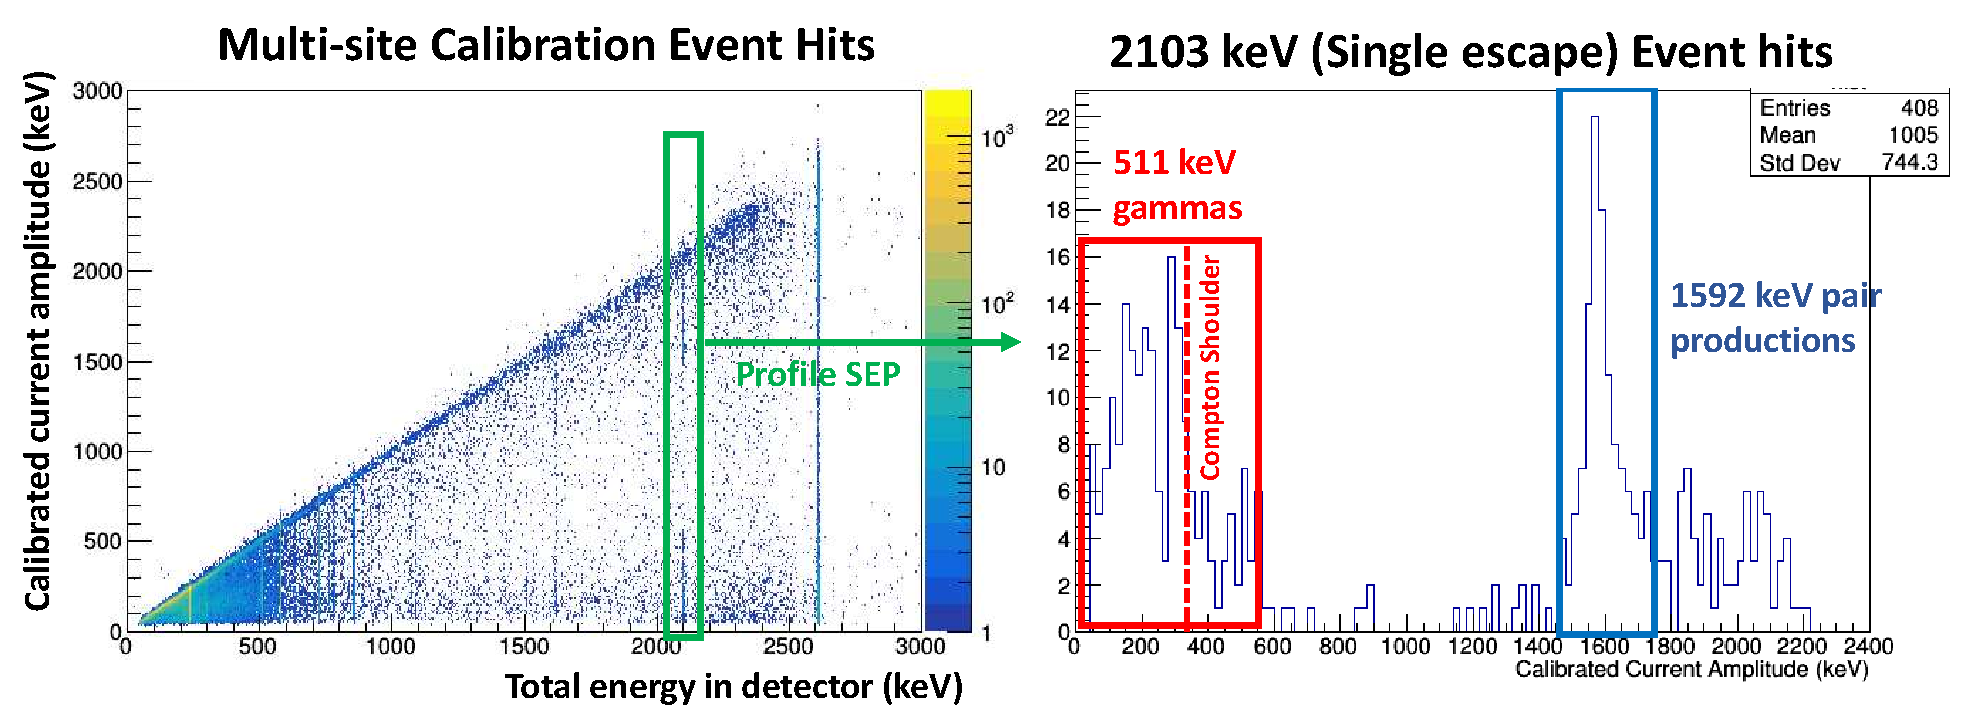
\includegraphics[width=\textwidth]{decomposedspectrum}
  \caption[Decomposed SEP spectrum]{\label{fig:eventdecompspectrum}
    Left: A 2D spectrum showing the energy of individual sites in multi-site events from a \Th{228} calibration run, vs the total energy of the event.\\
    Right: A profile along the single escape peak (total energy 2103~keV). The expected features of a 1592~keV peak for the pair production site and a 511~keV Compton spectrum from the $\gamma$ are observable.
  }
\end{figure}
To demonstrate the effectiveness of this technique, we can look at an inherently multi-site event such as a single-escape event.
The single-escape peak produced by the \Tl{208} 2614~keV~$\gamma$ will consist of a 1592~keV pulse, produced by the site of the pair production, and additional sites that sum to 511~keV, produced by the annihilation $\gamma$.
Figure~\ref{fig:eventdecompspectrum} shows how these expected features can be extracted from SEP events in a \MJD\ calibration run.
Using this technique, we are able to identify the 1592~keV site in 44\% of SEP events, a number that could significantly improve with refinements to the algorithm.

Multi-site event decomposition would be useful in searching for \bbes\ events because these events are inherently multi-site.
The search presented here takes advantage of this by looking at multi-detector events; however, often the $\gamma$-rays in these events will not escape the source detector without losing at least some energy.
In this case, the event would not be visible using this search's detection signature, but would be visible by looking for individual sites that sum to the full $\gamma$ energy.
Based on simulations, 60\% of \tnbb\ to \SP{0}{+}{1} events have the full energy of at least one of the two $\gamma$s absorbed inside of Germanium detectors, which sets a much higher ceiling on the detection efficiency than the 2\% used in this document.
Using the 44\% of pair production sites tagged in SEP events as a proxy, it is imaginable that such a search could achieve a detection efficency of 20-25\%, a ten-fold improvement over the current search.
This would also increase the measured background rate significantly, by introducing single-detector multi-site backgrounds; furthermore, the poorer energy resolution for these events would necessitate a wider ROI.
Even so, this could produce a large gain in sensitivity.

\subsection{Searching for \bbes\ with LEGEND}
LEGEND-200 is preparing to begin operation in 2021, with lower backgrounds than the \MJD\ and \Gerda\ and a target exposure of ${\sim}1$~t-y (Section~\ref{sec:legend}).
In spite of this high exposure, however, many challenges remain for LEGEND-200 to offer a significantly improved result in the search for \bbes.
LEGEND-200 will use the \Gerda\ liquid argon shield, which carries disadvantages for a \bbes\ search due to higher backgrounds and lower detection efficiencies.
\Gerda\ Phase~II may find techniques to mitigate these disadvantages, and will likely publish a result soon.
In addition, LEGEND-200 is using the inverted coaxial detector geometry, which increases the mass of each detector, but as a result reduces the granularity of the detector array.
This will further reduce detection efficiency.
Finally, once the \bbes\ to the \SP{0}{+}{1} decay is discovered, it will act as the largest background for the \SP{2}{+}{1} decay, which will further limit sensitivity without finding a method to distinguish the two.
For these reasons, LEGEND-200 may struggle to significantly improve upon the final \MJD\ results without implementing many of the improvements mentioned in the previous section.

If LEGEND-200 succeeds in these improvements and manages a measurement with $>10\%$ detection efficiency that remains nearly background free, future measurements could feasibly have half-life sensitivities exceeding $10^{26}$~y.
This would almost certainly observe the \bbes\ to \SP{0}{+}{1} decay mode (and if it didn't that would be an interesting result in its own right!).
It would also begin to probe into the theoretical half-life predictions for the \SP{2}{+}{1} decay mode, with potentially interesting results regarding a Bosonic component of neutrinos (Section~\ref{sec:bosonicnus}, \cite{Tornow2010}).
With the same improvements and lower backgrounds, LEGEND-1000 may probe half-lives exceeding $10^{27}$~y, offering a strong possibility of observing \tnbb\ to the \SP{2}{+}{1} excited state.
Finally, under the optimistic scenario that LEGEND-200 discovers \znbb, LEGEND-1000 may begin a search for \znbb\ to excited states, with implications toward understanding the underlying mechanism for \znbb\ decay and the Majorana nature of neutrino mass.

\onlyinsubfile{
  \bibliographystyle{unsrt}
  \bibliography{../main}
}

\end{document}
